\chapter{Experimenty}

V následující sekci ukážem několik experimentů, které jsme provedli s pomocí naší implementace. Experimenty budou vždy porovnávat několik hyper parametrů evolučního algoritmu a graficky ukážou fitness nejlepšího nalezeného jedince v závislosti na počtu vyhodnocení fitness funkce. Kromě ukázky z batohem pokaždé ukážeme nalevo minimální vzdálenost od cíle a napravo cenu mostu. Jako prostředí simulace jsme zvolili vždy pouze $1.$ úroveň. Pro každý experiment a každou zmíněnou kombinaci hypermarametrů jsme provedli $5$ běhu a jejich výsledek zprůměrovali. Na obrázcích jsme tak znázornili také $95\%$ konfidenční interval. Všechny experimenty jsme provedli na procesoru \texttt{AMD Ryzen 5 4500U with Radeon Graphics}. Vyhodnocování fitness jsme paralelizovali na všech $6$ jádrech procesoru.

\section{Jednoduchý příklad s batohem}

Experiment demonstruje výsledky běhu jednoduchého evolučního algoritmu na známém problému batohu, jak bylo představeno v sekci o problému batohu \ref{batoh}. Výsledky tohoto experimentu jsou prezentovány na obrázku \ref{exp:1}. Celková doba běhu jednoho experimentu byla přibližně $1$ minuta.

Z výsledků můžeme vidět, že běh poměrně rychle zkonvegroval. Už po $50$ generacích nelze pozorovat téměř žádné zlepšení. Zda jsem našli doopravdy optimální řešení bohužel nemužeme ověřit.

\begin{figure}[p]\centering
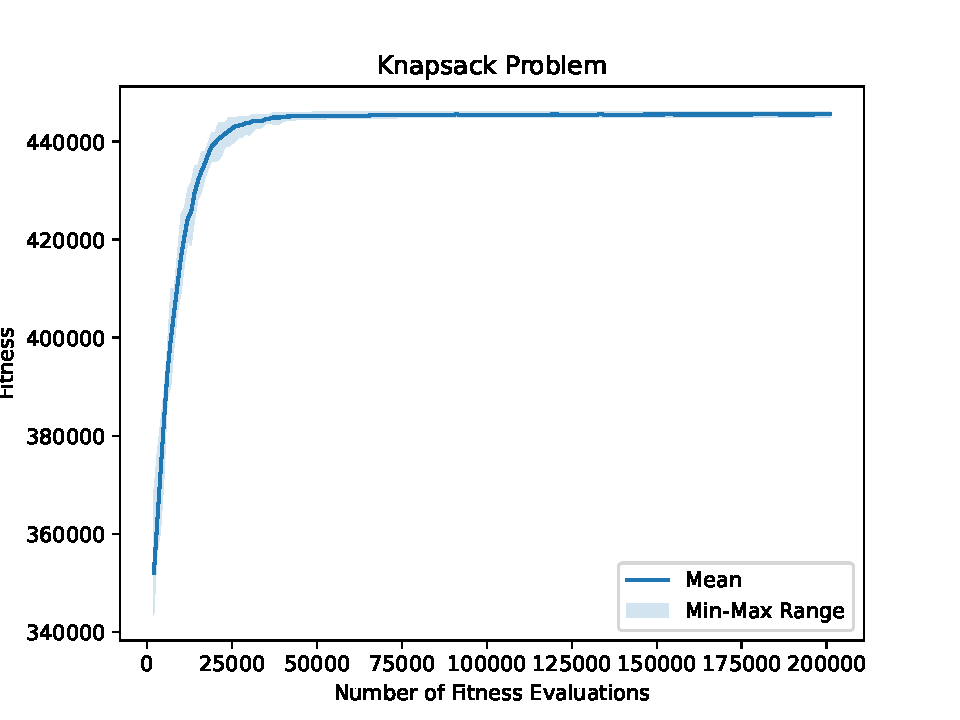
\includegraphics{img/knap}
\caption{Fitness nejlepšího jedince v závislosti na počtu vyhodnocení fitness funkce. Průměr $5$ běhů s $95\%$ konfidenčním intervalem. Velikost populace=$1000$, počet generací=$200$, p. mutace=$1/n$, p. křížení=$1$}
\label{exp:1}

\end{figure}


\section{Naivní přístup}

V tomto experimetu chceme ukázat, jakých výsledků lze dosáhnout pomocí jednoduchého kódování jedince. Z podstaty experimentu jsme se rozhodli vyzkoušet pouze jednu sadu hyperparametrů. Výsledek můžeme vidět na obrázku \ref{exp:2}. Doba jednoho běhu byla přibližně $11$ minut.

I přes jednoduchost našeho kódování se nám podařilo najít obstojný most. Tento postup bohužel ale vždy příliš brzy zkonverguje a tak se nám nedaří úroveň vyřešit.

\begin{figure}[p]\centering
\includegraphics[width=\linewidth]{img/simple}
\caption{Fitness nejlepšího jedince s jednoduchým kódováním v závislosti na počtu vyhodnocení fitness funkce. Nalevo minimální vzdálenost, napravo cena mostu. Průměr $5$ běhů s $95\%$ konfidenčním intervalem. Velikost populace=$250$, počet generací=$200$, p. mutace=$1/n$, p. křížení=$1$, délka jedince=$20$}
\label{exp:2}
\end{figure}


\section{Různé rozměry populace} \label{sizes}

Zkoumali jsme vliv různých kombinací velikosti populace a počtu generací na výkon algoritmu. Pro kódování jedinců jsme použili polární kódování. Výsledky jsou zobrazeny na obrázku \ref{exp:3}. Doba trvání jednoho běhu byla přibližně $11$ minut.

Z výsledků lze odvodit, že lepší fitness můžeme dosáhnout tím, že zvýšíme počet generací na úkor velikosti populace.

\begin{figure}[p]\centering
\includegraphics[width=\linewidth]{img/polar-pop}
\caption{Fitness nejlepšího jedince s polárním kódováním v závislosti na počtu vyhodnocení fitness funkce. Nalevo minimální vzdálenost, napravo cena mostu. Průměr $5$ běhů s $95\%$ konfidenčním intervalem. Velikost populace značená \emph{size}, počet generací značný \emph{gens}, p. mutace=$1/n$, p. křížení=$1$}
\label{exp:3}
\end{figure}

\section{Různé délky jedince}

Experimentovali jsme s různými délkami genomu pro jedince s polárním kódováním. Výsledky tohoto experimentu můžeme vidět na obrázku \ref{exp:35}. Délka běhu se lišila v závislosti na délce genomu, ale nepřesáhla $15$ minut.

Výsledky tohoto experimentu poukazují na důležitost výběru délky genomu jedince. Příliš krátký genom má za následek nedostatečnou schopnost jedince konstruovat kvalitní řešení, zatímco nadměrná délka vede k nadměrné hmotnosti a zhroucení celého mostu.

\begin{figure}[p]\centering
\includegraphics[width=\linewidth]{img/polar-len}
\caption{Fitness nejlepšího jedince s polárním kódováním v závislosti na počtu vyhodnocení fitness funkce. Nalevo minimální vzdálenost, napravo cena mostu. Průměr $5$ běhů s $95\%$ konfidenčním intervalem. Velikost populace=$250$, počet generací=$200$, p. mutace=$1/n$, p. křížení=$1$, délka jedince značí \emph{l}}
\label{exp:35}
\end{figure}

\section{Vylepšená fitness funkce}

Cílem tohoto experimentu je prozkoumat, zda vylepšená fitness funkce může zlepšit celkový výsledek algoritmu. Zkusili jsme několik různých vah $\alpha, \beta$ pro penalizace ve fitness funkci pro jedince s polárním kódováním. Výsledek toho experimenty můžeme vidět na obrázku \ref{exp:4}. Doba jednoho běhu byla přibližně $11$ minut.

Bylo překvapivé, že náš návrh fitness funkce s penalizacemi nepomohl nalezení lepšího mostu. Z výsledků experimentů se zdá, že algoritmus místo toho, optimalizoval strukturu mostu, přestane úplně most stavit. Docílí se tak minimální penalizace a tudíž i lepší fitness a předčasně zkonvergujeme do lokálního minima. 

\begin{figure}[p]\centering
\includegraphics[width=\linewidth]{img/impolar}
\caption{Fitness nejlepšího jedince s polárním kódováním a vylepšenou fitness funkcí v závislosti na počtu vyhodnocení fitness funkce. Nalevo minimální vzdálenost, napravo cena mostu. Průměr $5$ běhů s $95\%$ konfidenčním intervalem. Velikost populace=$250$, počet generací=$200$, p. mutace=$1/n$, p. křížení=$1$, délka jedince=$20$, parametry $\alpha, \beta$ značí \emph{alpha, beta}}
\label{exp:4}
\end{figure}


\section{Populace s elitismem} 

V tomto experimentu jsme vyzkoušeli jaký vliv má elitismus na běh algoritmu. Zkusili jsme několik úrovní elitismu pro jedince s polárním kódováním, jejich rozdíly můžme vidět na obrázku \ref{exp:5}. Doba jednoho běhu byla přibližně $11$ minut.

V tomto experimentu si můžeme všimnout, že elitismus tolik nepomáhá. Zajímavé je si všimnout i toho, že pokud nastavíme sílu elitismu vysoko, můžeme dosáhnout ještě lepších výsledků než bez elitismu. Tím se nám znovu potvrzuje náš závěr z experimentu \ref{sizes}, že můžeme dosáhnout lepší když budeme upřednostňovat exploataci.

\begin{figure}[p]\centering
\includegraphics[width=\linewidth]{img/elit}
\caption{Fitness nejlepšího jedince s polárním kódováním v závislosti na počtu vyhodnocení fitness funkce. Nalevo minimální vzdálenost, napravo cena mostu. Průměr $5$ běhů s $95\%$ konfidenčním intervalem. Velikost populace=$250$, počet generací=$200$, p. mutace=$1/n$, p. křížení=$1$, sílu elitismu značí $elit$}
\label{exp:5}
\end{figure}


\section{Ztěžující se fitness} \label{inc}

V následující experimentu vyzkoušíme, zda pomáhá postupné zvyšování obtížnosti problému. Počáteční vzdálenost břehů je nastavena na $10\%$ původní vzdálenosti. Vyzkoušeli jsme různé hranice průměrné fitness populace nutné na zvýšení obtížnosti. Také jsme zkusili různé velikosti kroků ztěžování. Použili jsme polární kódování jedince. Výsledek tohoto experimentu můžeme vidět na obrázke \ref{exp:6}. Doba jednoho běhu byla přibližně $11$ minut.

Bohužel se nám touto metodou nepodařil dosáhnout požadovaných výsledků. Z podstaty metody ale můžeme odvodit, že algoritmus nestihl zkonvergovat k suboptimálnímu řešení, takže je možné, že kdybychom měli k dispozici více výpočetního času, mohli bychom mnohem lepších řešení.

\begin{figure}[p]\centering
\includegraphics[width=\linewidth]{img/inc}
\caption{Fitness nejlepšího jedince s polárním kódováním v závislosti na počtu vyhodnocení fitness funkce. Nalevo minimální vzdálenost, napravo cena mostu. Průměr $5$ běhů s $95\%$ konfidenčním intervalem. Velikost populace=$250$, počet generací=$200$, p. mutace=$1/n$, p. křížení=$1$, hranice pro zvýšení obtížnosti značí \emph{avg}, velikost kroku \emph{increase}}
\label{exp:6}
\end{figure}

\section{Grafové kódování}

Několik následující experimentů budou zkoumat efektivitu algoritmu s jedinci, kteří použivají grafové kódování. Nejdříve jsme zkoumali, jaký vliv má počet vrcholů na kvalitu jedinců. Výsledky experimentu jsou zobrazeny na obrázku \ref{exp:7}. Doba běhu se lišila v závislosti na délce jedince, ale nebyla delší než $21$ minut.

Je těžké z výsledků tohoto experimentu něco odvodit. Počet hran v genomu jedince se můžem mutacemi měnit tak na počátečním počtu vrcholů (tudíž i hran) příliš nezáleží.

\begin{figure}[p]\centering
\includegraphics[width=\linewidth]{img/graph}
\caption{Fitness nejlepšího jedince s grafovým kódování v závislosti na počtu vyhodnocení fitness funkce. Nalevo minimální vzdálenost, napravo cena mostu. Průměr $5$ běhů s $95\%$ konfidenčním intervalem. Velikost populace=$250$, počet generací=$200$, p. mutace vrcholu=$1/n$, p.mutace hrany = $1/n$, p. křížení=$1$, \emph{nodes} značí různé počty použitých vrcholů}
\label{exp:7}
\end{figure}


\section{Grafové kódování a stěžující se fitness}

Tento experiment rozšiřuje předchozí testování grafového kódování o postupné ztěžování problému během evoluce. Cílem bylo zjistit, zda kombinace grafového kódování a postupného zvyšování obtížnosti může vést k robustnější adaptaci jedinců na složitější úkoly. Výsledek tohoto experimentu můžeme vidět na obrázku \ref{exp:8}. Doba jednoho běhu byla přibližně $20$ minut.

Z tohoto experimentu můžeme odvodit podobné závery jako z experimentu~\ref{inc}. \xxx{závěr tohoto experimentu musím dopsat až doběhne}

\begin{figure}[p]\centering
\includegraphics[width=\linewidth]{img/graph-inc}
\caption{Fitness nejlepšího jedince s grafovým kódování v závislosti na počtu vyhodnocení fitness funkce. Nalevo minimální vzdálenost, napravo cena mostu. Průměr $5$ běhů s $95\%$ konfidenčním intervalem. Velikost populace=$250$, počet generací=$200$, p. mutace=$1/n$, p. křížení=$1$, hranice pro zvýšení obtížnosti značí \emph{avg}, velikost kroku \emph{increase}}
\label{exp:8}
\end{figure}


\section{Lepší inicializace jedince}

Poslední experiment se zaměřuje na vliv vylepšené inicializace jedinců s grafovým kódování na celkový výkon evolučního algoritmu. Vyzkoušeli jsme různé hodnoty $\omega$. Výsledky jsou ilustrovány na obrázku \ref{exp:9}. Doba běhu se mírně lišila v závislosti na metodě inicializace, ale průměrně trvala 10 minut.

Tento experiment ukazuje, že tímto způsobem inicializace vpodstatě těžkou část problému, tedy dostat vozidlo z jedné strany na druhou, vyřešíme neoptimálním návrhem. Algoritmu pak zbývá pouze tento návrh lehce modifikovat mutacemi a křížením, což se jeví jako mnohem lepší postup, než se nejprve snažit najít optimální strukturu mostu. 

\begin{figure}[p]\centering
\includegraphics[width=\linewidth]{img/init}
\caption{Fitness nejlepšího jedince s grafovým kódování a vylepšenou inicializací v závislosti na počtu vyhodnocení fitness funkce. Nalevo minimální vzdálenost, napravo cena mostu. Průměr $5$ běhů s $95\%$ konfidenčním intervalem. Velikost populace=$250$, počet generací=$200$, p. mutace vrcholu=$1/n$, p.mutace hrany = $1/n$, p. křížení=$1$, \emph{omega} značí různé hodnoty $\omega$}
\label{exp:9}
\end{figure}


\begin{figure}[p]\centering
\includegraphics[width=\linewidth]{img/comp}
\caption{Porovnání různých kódování jedinců. \emph{t} značí typ jedince}
\label{zaver:1}
\end{figure}


\section{Přenesení do Poly Bridge}

V tomto exeperimentu ukážeme, jak nejlepší nalezená řešení pomocí evolučních algoritmu fungují ve hře. Na obrázcích \ref{exp:lvl1}, \ref{exp:lvl2}, \ref{exp:lvl3} a \ref{exp:lvl4} můžeme vidět porovnání nalezených řešení v simulaci, ve hře a řešení navrhnutá člověkem. V tabulce \ref{tab:2} můžeme vidět, zda se nám úroveň podařilo vyřešit evolučním algoritmem a cenu navrženého mostu. Pro hledání řešení jsme pro všechny úrovně zvolili grafové kódování jedince s vylepšenou inicializací ($\omega=1$), velikostí populace $size=500$, počet generací $gens=1000$ s nízkým elitismem $0.02$. Takto nastavený algorimtus jsme pro každou úroveň zopakovali $5$krát a vybrali nejlepší řešení. Doba jednoho běhu byla zhruba $25$ minut.

Evolučním algoritmem se nám podařilo vyřešit $3$ ze $4$ úrovní, u dvou z nich algoritmus navrhnul levnější řešení než člověk.

\begin{table}[b!]
\centering
\begin{tabular}{lccc}
\toprule
\textbf{Úroveň} & \textbf{Vyřešeno algoritmem} & \textbf{Cena \$} & \textbf{Cena lidského řešení \$} \\
\midrule
\emph{Úroveň 1} & Ano &  4133 & 3954 \\
\emph{Úroveň 2} & Ano &  3262 & 5752 \\
\emph{Úroveň 3} & Ano &  5544 & 5736 \\
\emph{Úroveň 4} & Ne  &  3788 & 4821 \\
\bottomrule
\end{tabular}
\caption{Ceny mostů navržených evolučním algoritmem v porovnání s lidským řešením}
\label{tab:2}
\end{table}


\begin{figure}[ht]
    \centering
    \begin{minipage}{0.32\textwidth}
        \centering
        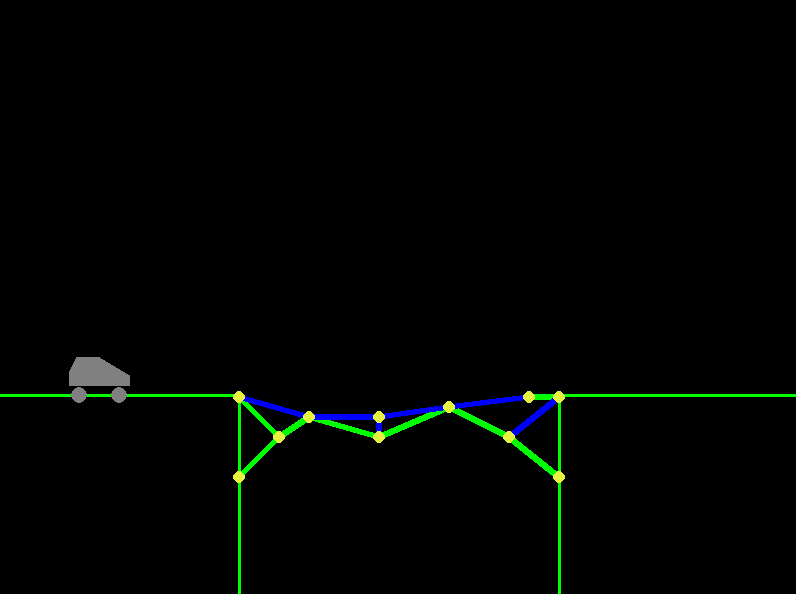
\includegraphics[width=\linewidth]{img/lvl1-sim-ea}
    \end{minipage}\hfill
    \begin{minipage}{0.32\textwidth}
        \centering
        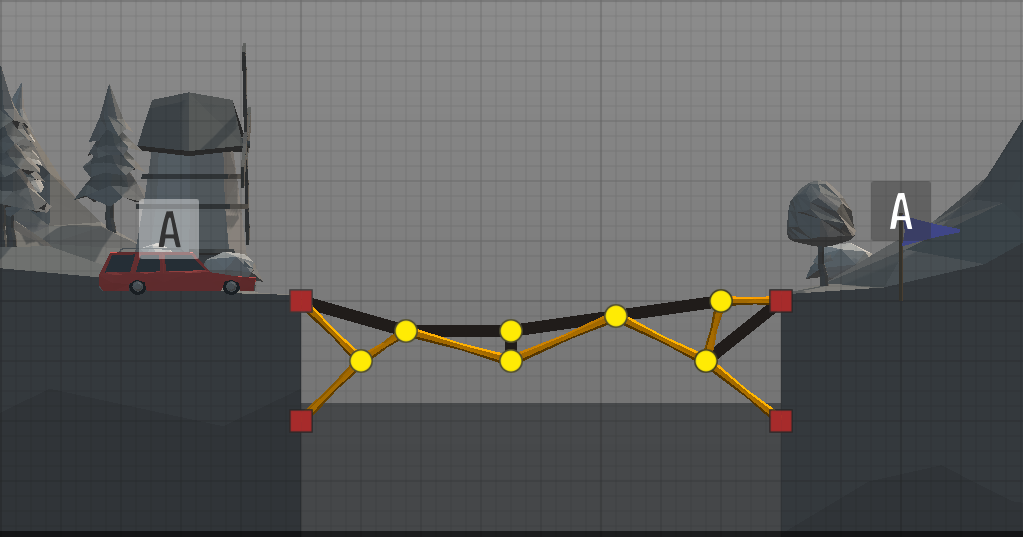
\includegraphics[width=\linewidth]{img/lvl1-poly-ea}
    \end{minipage}
    \begin{minipage}{0.32\textwidth}
        \centering
        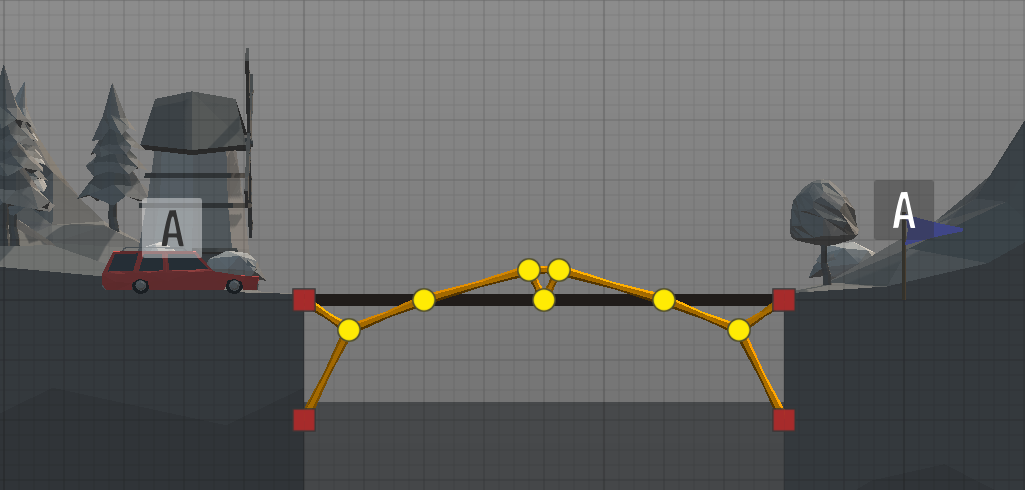
\includegraphics[width=\linewidth]{img/lvl1-poly-human}
    \end{minipage}
    \caption{Řešení první úrovně navrhnuté evolučním algoritmem. Nalevo je řešení zobrazené v simulaci, uprostřed ve hře, napravo řešení navrhnuté člověkem}
    \label{exp:lvl1}
\end{figure}

\begin{figure}[ht]
    \centering
    \begin{minipage}{0.32\textwidth}
        \centering
        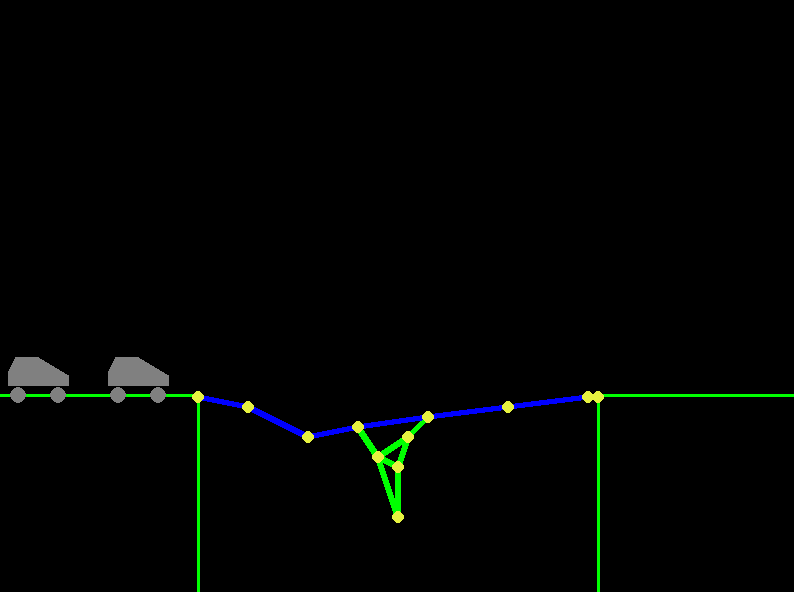
\includegraphics[width=\linewidth]{img/lvl2-sim-ea}
    \end{minipage}\hfill
    \begin{minipage}{0.32\textwidth}
        \centering
        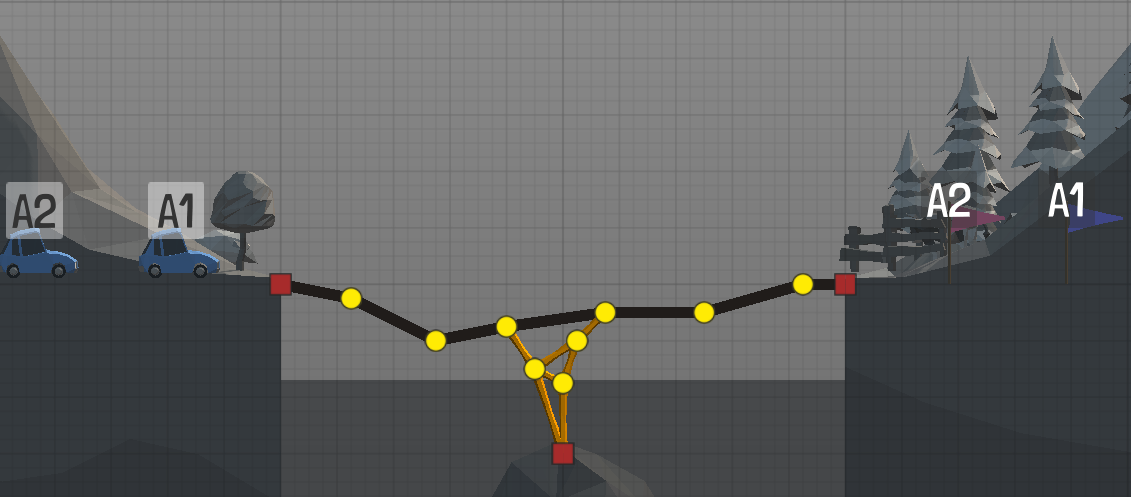
\includegraphics[width=\linewidth]{img/lvl2-poly-ea}
    \end{minipage}
    \begin{minipage}{0.32\textwidth}
        \centering
        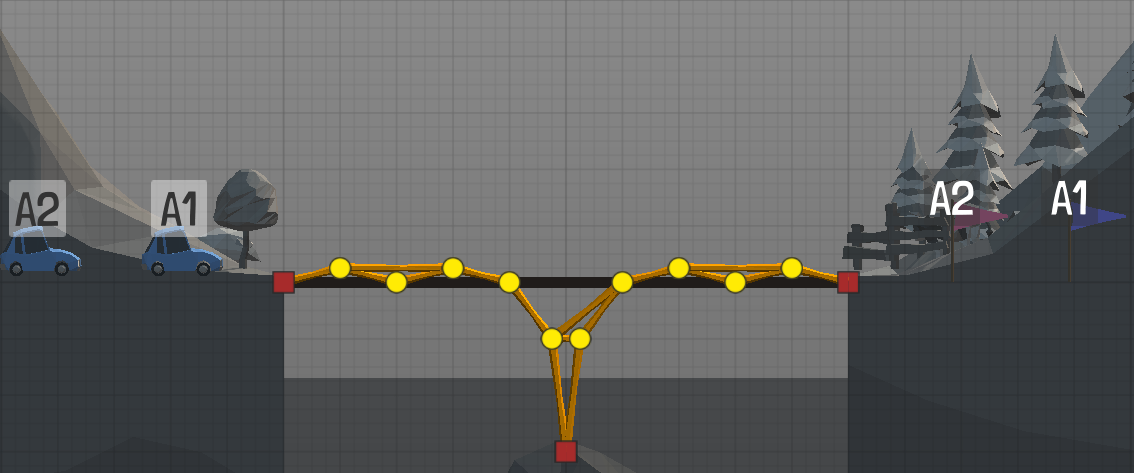
\includegraphics[width=\linewidth]{img/lvl2-poly-human}
    \end{minipage}
    \caption{Řešení druhé úrovně navrhnuté evolučním algoritmem. Nalevo je řešení zobrazené v simulaci, uprostřed ve hře, napravo řešení navrhnuté člověkem}
    \label{exp:lvl2}
\end{figure}

\begin{figure}[ht]
    \centering
    \begin{minipage}{0.32\textwidth}
        \centering
        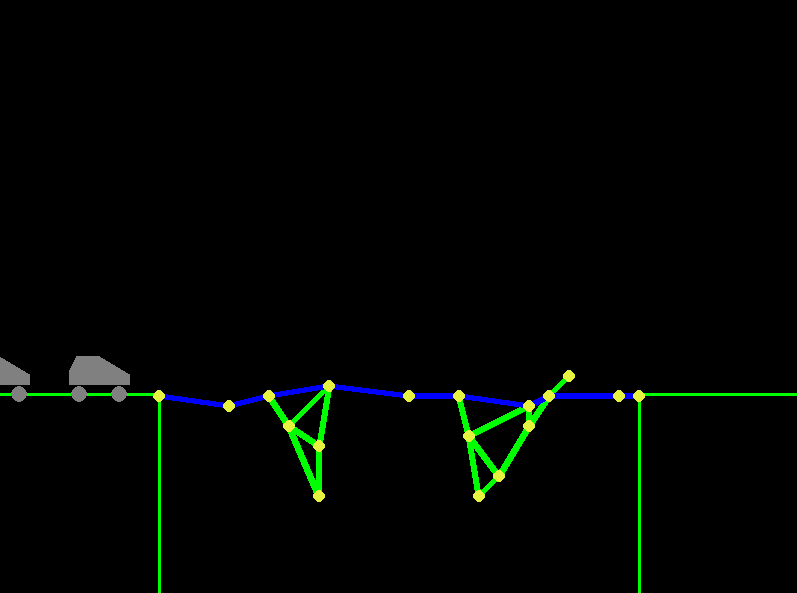
\includegraphics[width=\linewidth]{img/lvl3-sim-ea}
    \end{minipage}\hfill
    \begin{minipage}{0.32\textwidth}
        \centering
        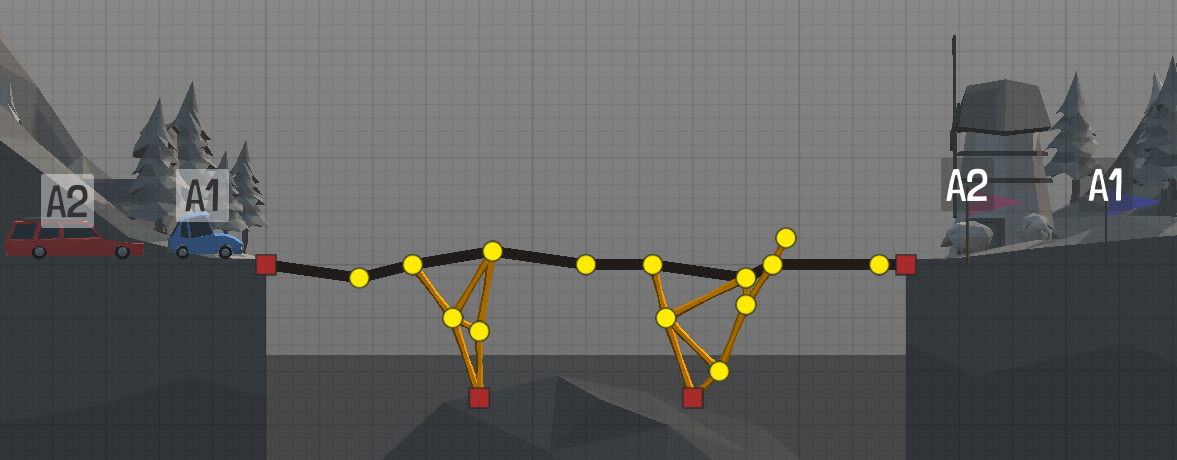
\includegraphics[width=\linewidth]{img/lvl3-poly-ea}
    \end{minipage}
    \begin{minipage}{0.32\textwidth}
        \centering
        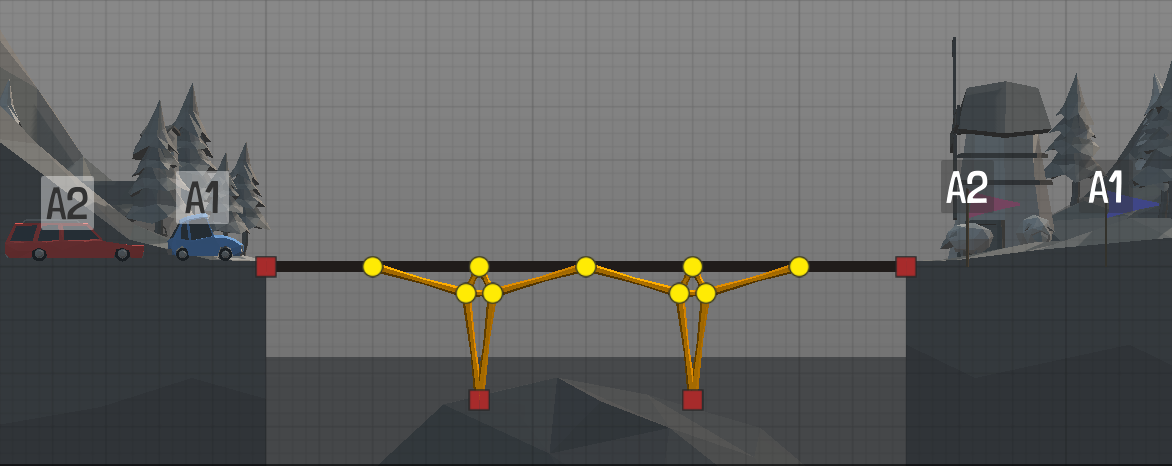
\includegraphics[width=\linewidth]{img/lvl3-poly-human}
    \end{minipage}
    \caption{Řešení třetí úrovně navrhnuté evolučním algoritmem. Nalevo je řešení zobrazené v simulaci, uprostřed ve hře, napravo řešení navrhnuté člověkem}
    \label{exp:lvl3}
\end{figure}

\begin{figure}[ht]
    \centering
    \begin{minipage}{0.32\textwidth}
        \centering
        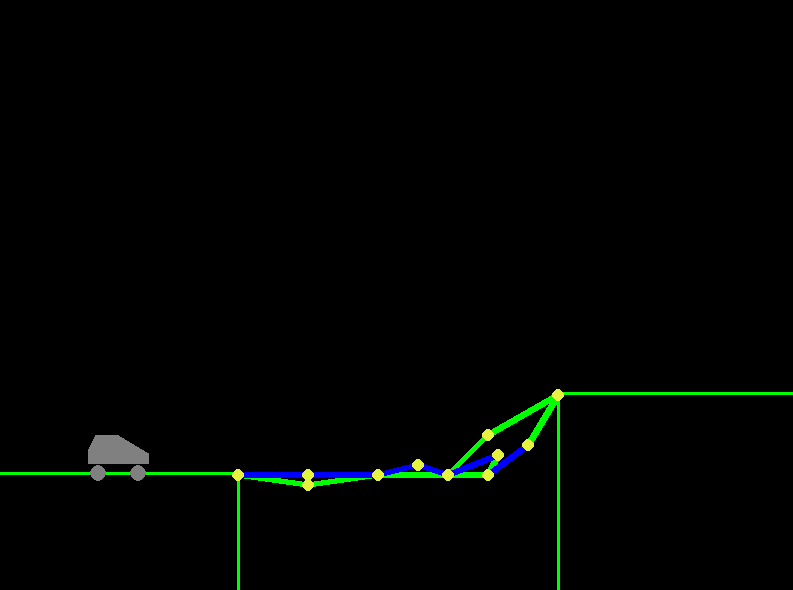
\includegraphics[width=\linewidth]{img/lvl4-sim-ea}
    \end{minipage}\hfill
    \begin{minipage}{0.32\textwidth}
        \centering
        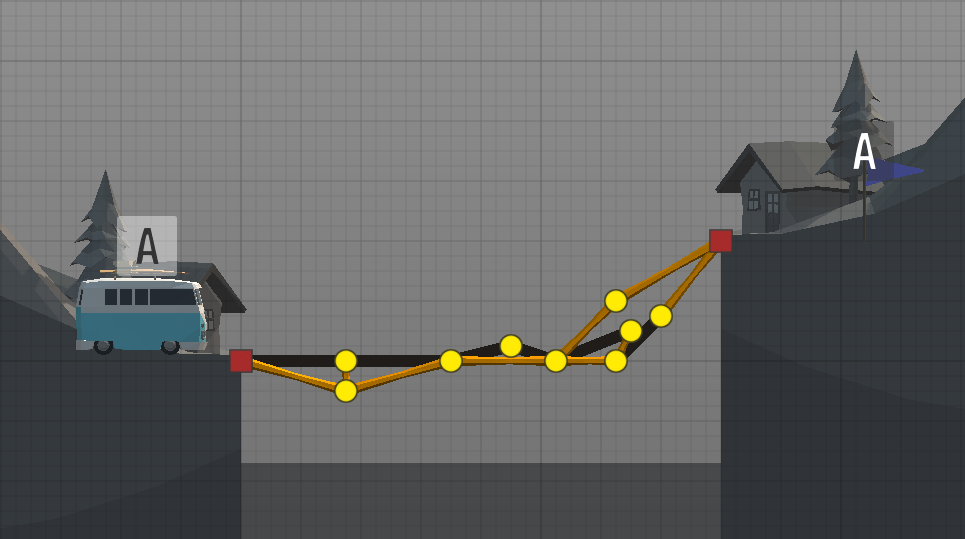
\includegraphics[width=\linewidth]{img/lvl4-poly-ea}
    \end{minipage}
    \begin{minipage}{0.32\textwidth}
        \centering
        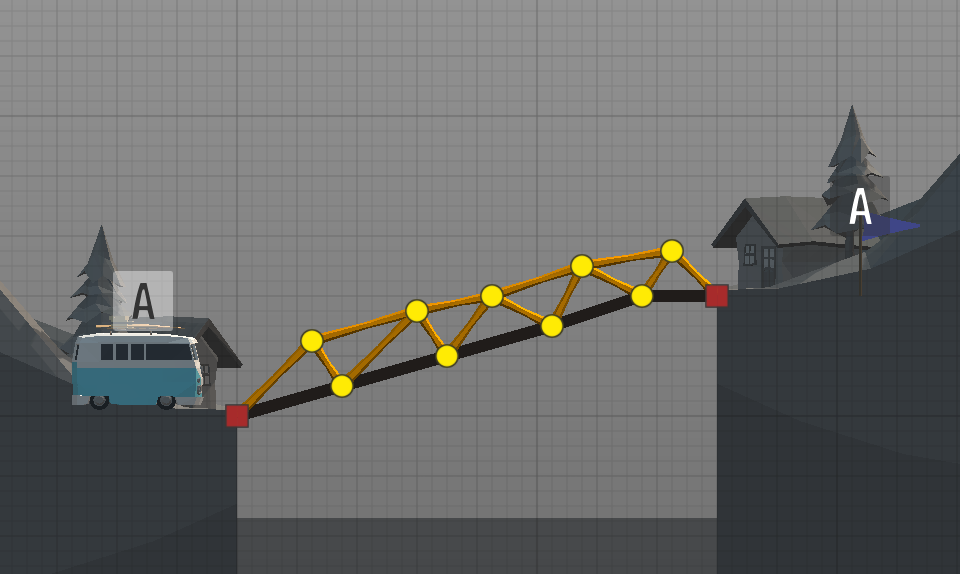
\includegraphics[width=\linewidth]{img/lvl4-poly-human}
    \end{minipage}
    \caption{Řešení čtvrté úrovně navrhnuté evolučním algoritmem. Nalevo je řešení zobrazené v simulaci, uprostřed ve hře, napravo řešení navrhnuté člověkem}
    \label{exp:lvl4}
\end{figure}


